\documentclass[border=8pt]{standalone}
\usepackage[T1]{fontenc}
\usepackage{xcolor}
\usepackage{amsmath}
\usepackage{siunitx}
\usepackage{tikz}
\usetikzlibrary{arrows.meta,positioning,shapes.geometric,calc,fit,backgrounds}
\usepackage[siunitx,american]{circuitikz}
\usepackage{mathptmx}
\definecolor{ink}{HTML}{14202B}
\definecolor{slate}{HTML}{24394B}
\definecolor{amber}{HTML}{C9781E}
\definecolor{amberlight}{HTML}{FBEBD3}
\definecolor{teal}{HTML}{3E7F8C}
\definecolor{paper}{HTML}{F6F3EC}
\definecolor{muted}{HTML}{5E6974}

\newcommand{\code}[1]{\texttt{#1}}
\tikzset{
  blk/.style={draw=slate,rounded corners=3pt,fill=white,align=center,font=\small,minimum height=0.9cm,text width=3.3cm},
  hub/.style={draw=amber,line width=1.1pt,rounded corners=4pt,fill=amberlight,align=center,font=\small},
  arr/.style={-{Stealth[length=2.2mm]},draw=slate,line width=0.7pt},
  stp/.style={draw=slate,rounded corners=3pt,fill=white,align=center,font=\small,minimum height=1.1cm,text width=4.2cm},
}

\begin{document}
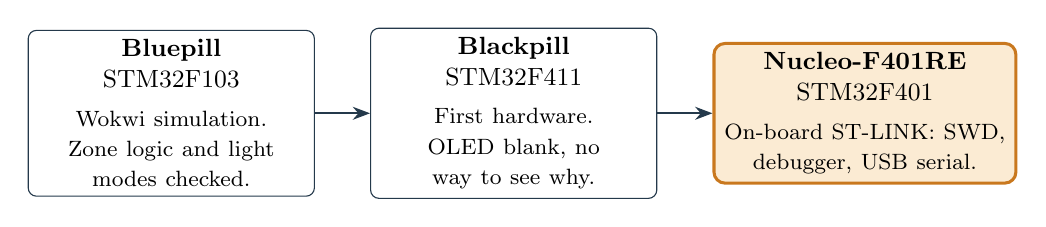
\begin{tikzpicture}[node distance=0.7cm]
\node[blk,text width=3.4cm] (bp) {\textbf{Bluepill}\\STM32F103\\[3pt]\footnotesize Wokwi simulation. Zone logic and light modes checked.};
\node[blk,text width=3.4cm,right=of bp] (bk) {\textbf{Blackpill}\\STM32F411\\[3pt]\footnotesize First hardware. OLED blank, no way to see why.};
\node[hub,text width=3.6cm,minimum height=0.9cm,right=of bk] (nu) {\textbf{Nucleo-F401RE}\\STM32F401\\[3pt]\footnotesize On-board ST-LINK: SWD, debugger, USB serial.};
\draw[arr] (bp) -- (bk);
\draw[arr] (bk) -- (nu);
\end{tikzpicture}
\end{document}
